%*************************************
% บทที่ 4
%*************************************
\chapterTitle{4}{ผลการดำเนินงาน}

\hspace*{1.3em}
ในการพัฒนา เว็บแอปพลิเคชันเพื่อการคอนฟิกด้วยวิธี NETCONF ผ่าน LLM ได้จัดทำโครงสร้างและการปรับแต่งระบบให้สอดคล้องกับมาตรฐานที่กำหนด ประกอบด้วยการจัดการอุปกรณ์ การสร้างและปรับใช้การกำหนดค่า การสำรองข้อมูล และการประมวลผลด้วย LLM
\section{ผลการดำเนินงาน}
\hspace*{1.3em}
รายละเอียดการทำงานของโปรแกรมผลการดำเนินงานในการจัดทำโครงงานเว็บแอปพลิเคชันเพื่อการคอนฟิกด้วยวิธี NETCONF ผ่าน LLM มีรายละเอียดดังนี้

\begin{figure}[H]
\centering
\adjustbox{frame, width=1.0\textwidth}{%สร้างกรอบของภาพ
    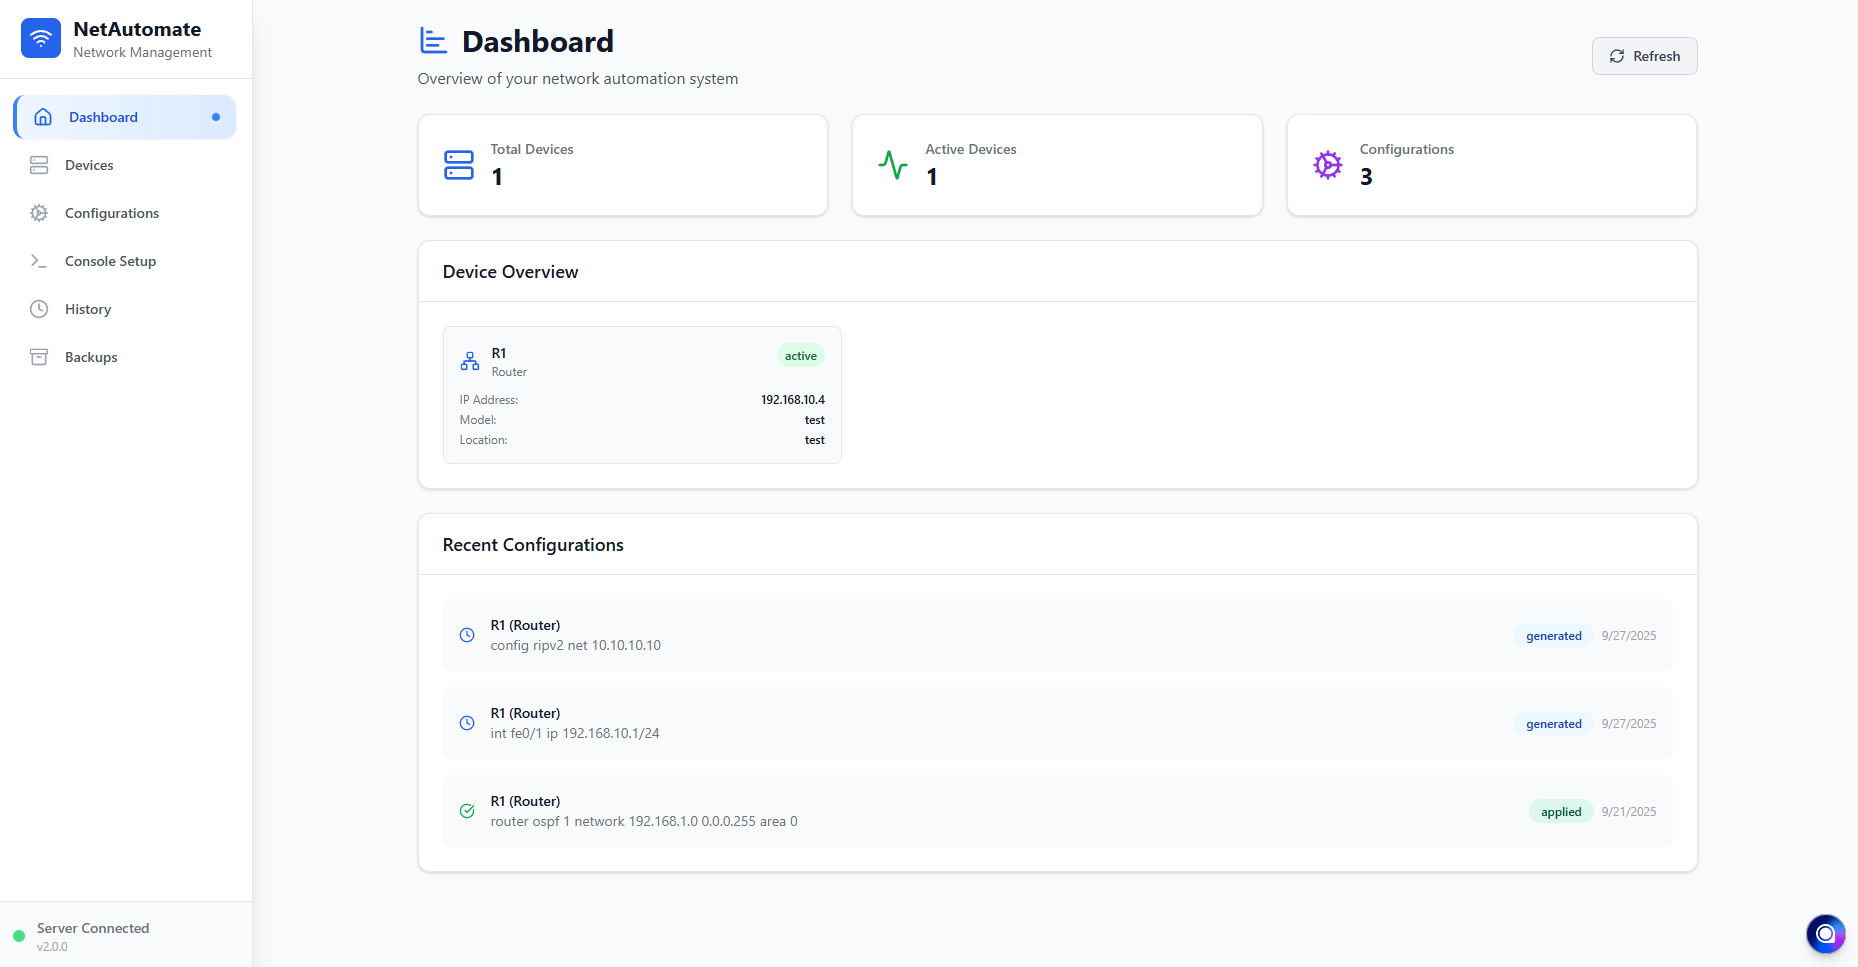
\includegraphics[width=1.0\textwidth]{Image/dashboard.png}
}
\caption{\fontSixTeen{หน้าจอ Dashboard}}
\label{fig4:Dashboard}
\end{figure}

\hspace*{1.3em} %ย่อหน้า
จากภาพที่ \ref{fig4:Dashboard} แสดงภาพรวมของระบบ ระบุจำนวนอุปกรณ์ที่เชื่อมต่ออยู่และจำนวน Configurations ที่มีอยู่ในระบบและแสดงรายรายละเอียดของอุปกรณ์ IP Address, Model, Location, Status และรายละเอียดของ Configurations 5 ครั้งล่าสุด


\begin{figure}[H]
\centering
\adjustbox{frame, width=1.0\textwidth}{%สร้างกรอบของภาพ
    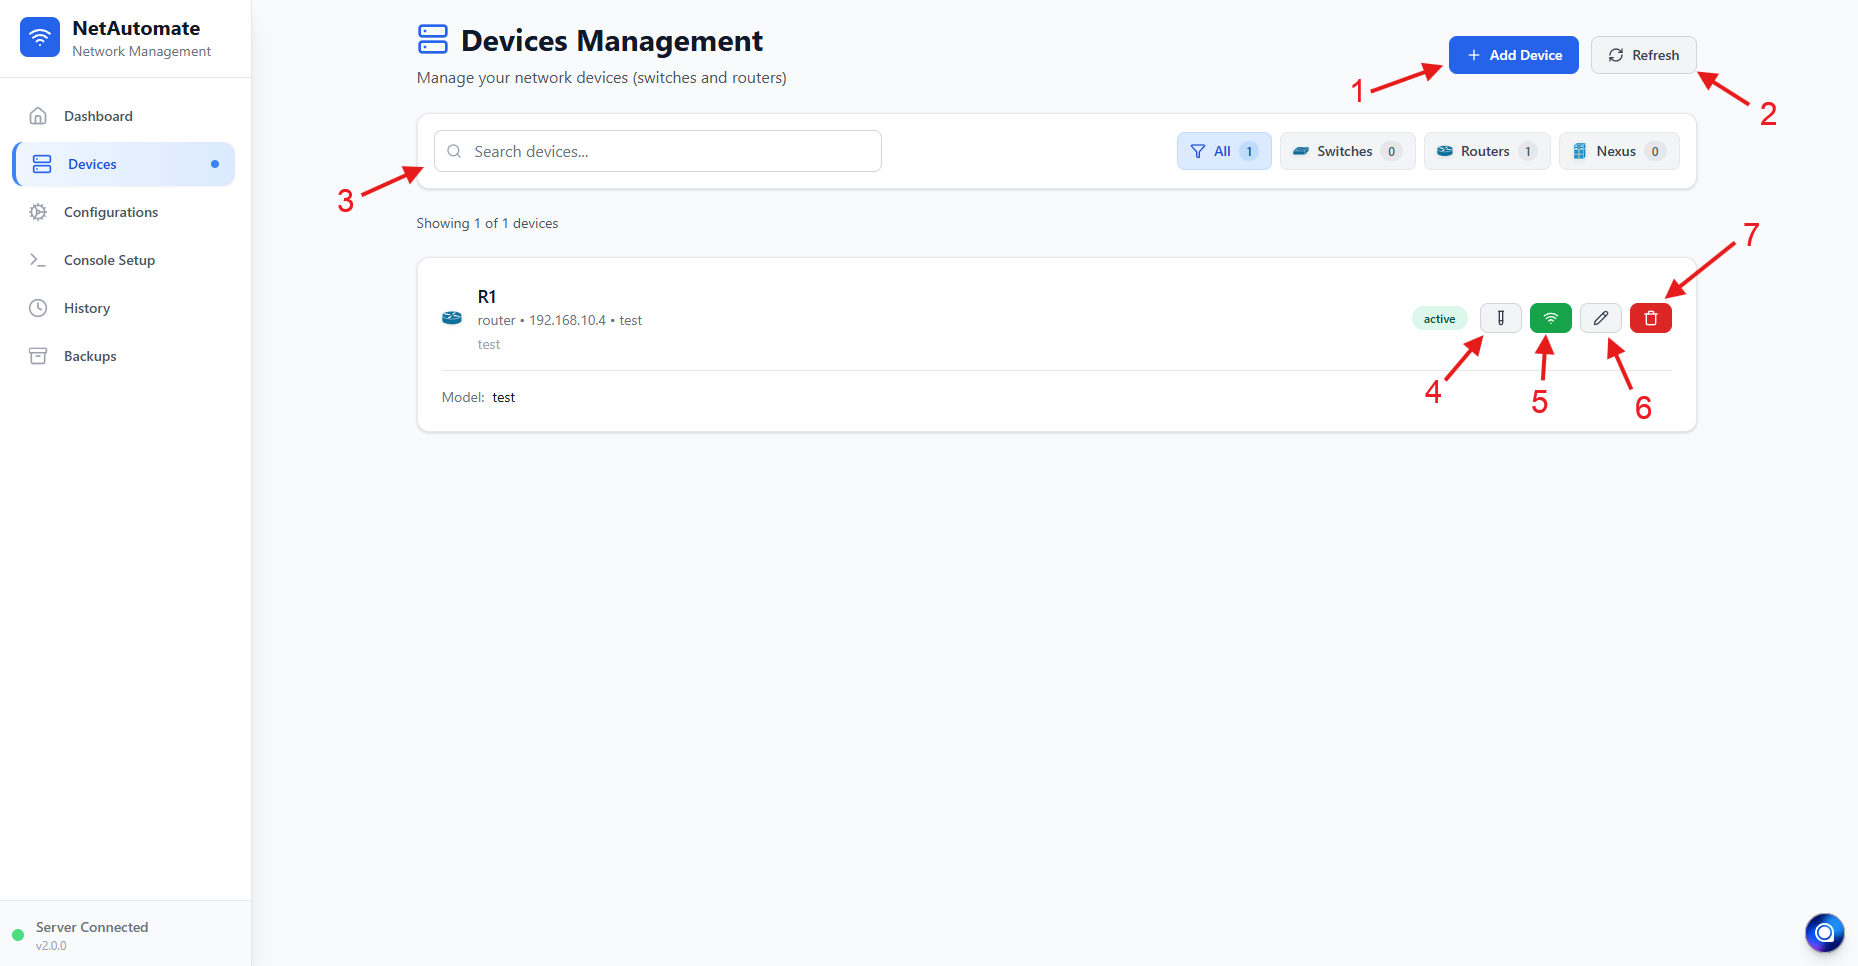
\includegraphics[width=1.0\textwidth]{Image/DeviceManage.png}
}
\caption{\fontSixTeen{หน้าจอ Device Management}}
\label{fig4:DeviceManage}
\end{figure}

\hspace*{1.3em} %ย่อหน้า
จากภาพที่ \ref{fig4:DeviceManage} แสดงหน้าจอสำหรับการจัดการอุปกรณ์ในระบบ ซึ่งประกอบด้วยฟิลด์ต่าง ๆ สำหรับกรอกข้อมูลเริ่มต้น ดังนี้

\hspace*{1.3em} %ย่อหน้า
หมายเลข 1 ปุ่ม Add Device สำหรับเพิ่มอุปกรณ์ใหม่เพื่อบันทึกข้อมูลอุปกรณ์ใหม่เข้าสู่ระบบ

\hspace*{1.3em}
หมายเลข 2 ปุ่มรีเฟรช (Refresh) เพื่อดึงข้อมูลอุปกรณ์ล่าสุดจากฐานข้อมูล

\hspace*{1.3em}
หมายเลข 3 ช่อง Search Bar สำหรับค้นหาอุปกรณ์

\hspace*{1.3em}
หมายเลข 4 ปุ่ม Test Connection ระหว่างอุปกรณ์กับเว็บแอปพลิเคชัน

\hspace*{1.3em}
หมายเลข 5 ปุ่ม Connection กับอุปกรณ์ผ่านโปรโตคอล SSH

\hspace*{1.3em}
หมายเลข 6 ปุ่ม Edit สำหรับแก้ไขข้อมูลของอุปกรณ์

\hspace*{1.3em}
หมายเลข 7 ปุ่ม Delete สำหรับลบอุปกรณ์ออกจากระบบ

\begin{figure}[H]
\centering
\adjustbox{frame, width=1.0\textwidth}{%สร้างกรอบของภาพ
    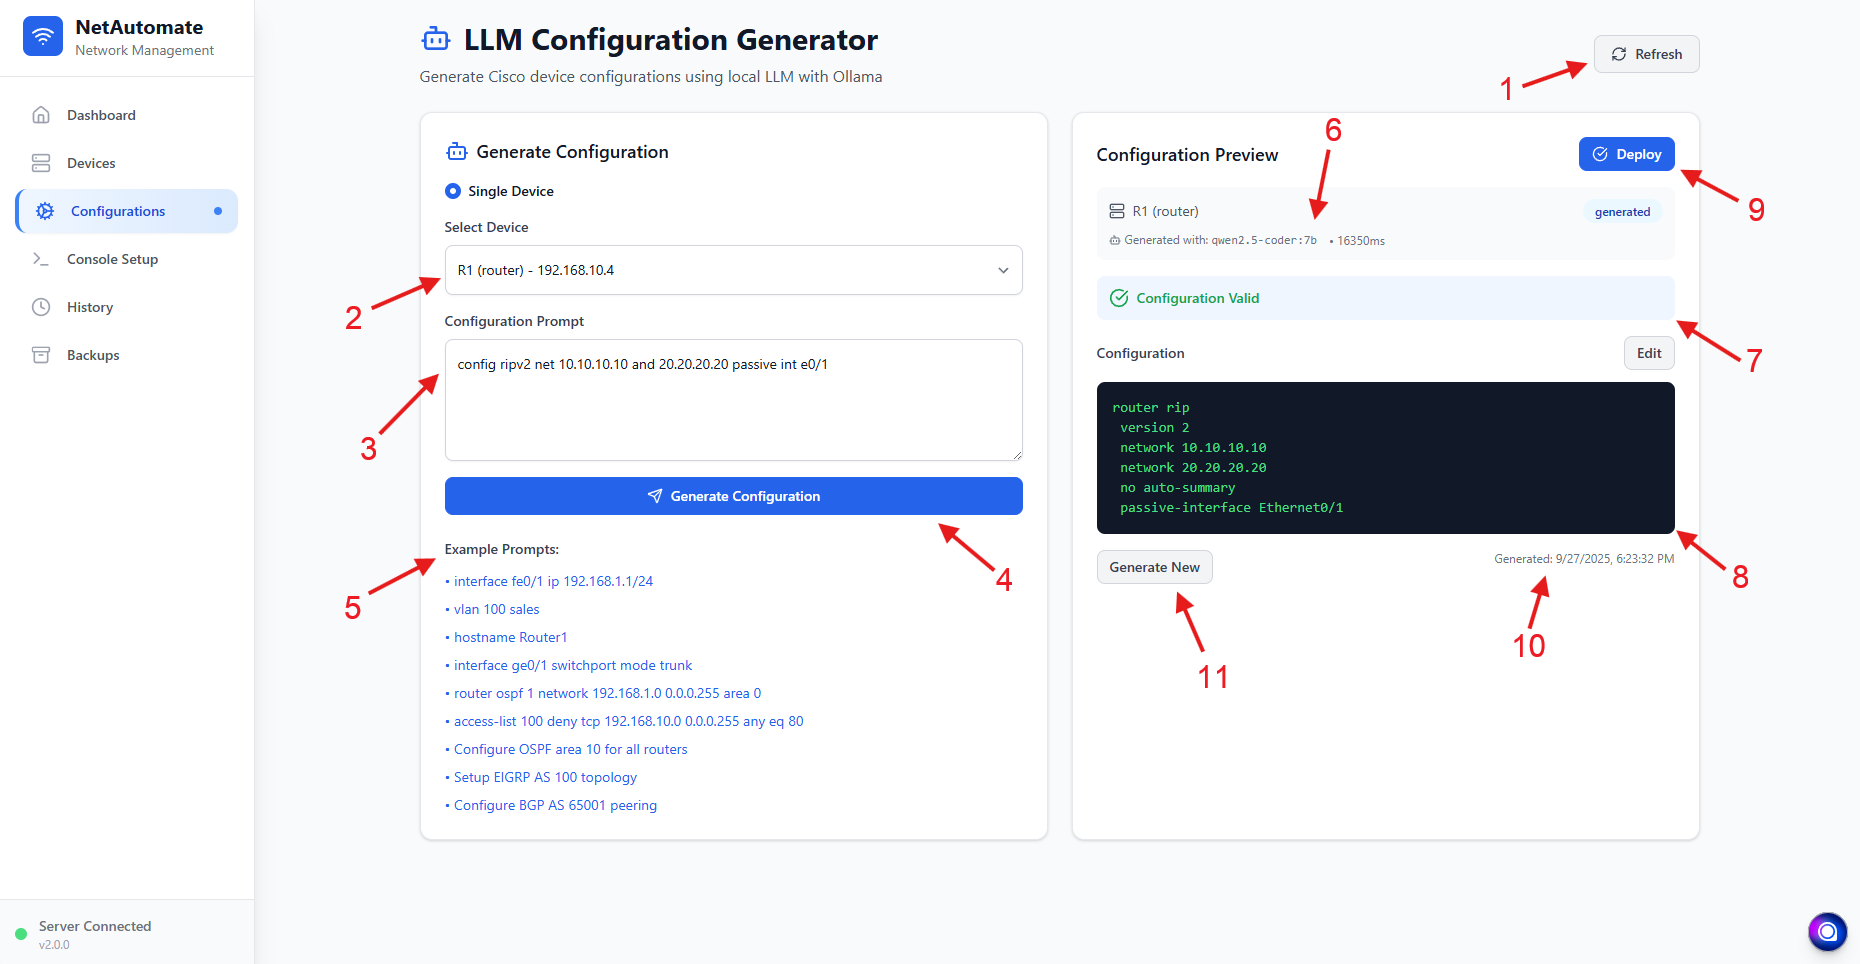
\includegraphics[width=1.0\textwidth]{Image/Configurations.png}
}
\caption{\fontSixTeen{หน้าจอ LLM Configuration Generator}}
\label{fig4:Configurations}
\end{figure}

\hspace*{1.3em} %ย่อหน้า
จากภาพที่ \ref{fig4:Configurations} แสดงหน้าจอสำหรับการจัดการ Configurations ในระบบ ซึ่งประกอบด้วยฟิลด์ต่าง ๆ สำหรับการกำหนดค่าอุปกรณ์ ดังนี้

\hspace*{1.3em} %ย่อหน้า
หมายเลข 1 ปุ่มรีเฟรช (Refresh) เพื่อดึงข้อมูลอุปกรณ์ล่าสุดจากฐานข้อมูล

\hspace*{1.3em}
หมายเลข 2 เลือกอุปกรณ์ที่ต้องการจะ Configurations (รองรับการเลือกหลายอุปกรณ์พร้อมกันในโหมด CLI ด้วย Checkbox พร้อม Select All)

\hspace*{1.3em}
หมายเลข 3 ช่องสำหรับใส่ Prompt ที่ต้องการให้ LLM สร้างคำสั่งการกำหนดค่าอุปกรณ์

\hspace*{1.3em}
หมายเลข 4 ปุ่ม Generate Configuration เพื่อให้ LLM สร้างคำสั่งการกำหนดค่าอุปกรณ์ (เมื่อเลือกหลายอุปกรณ์ ระบบจะสร้างคอนฟิกให้ทุกอุปกรณ์ที่เลือกพร้อมกัน)

\hspace*{1.3em}
หมายเลข 5 Example Prompt สำหรับตัวอย่างการใส่ Prompt

\hspace*{1.3em}
หมายเลข 6 ระบุรายละเอียดของ Model ที่ใช้และเวลาที่ใช้ในการสร้างคำสั่ง

\hspace*{1.3em}
หมายเลข 7 ระบุความถูกต้องของคำสั่งที่สร้างขึ้น

\hspace*{1.3em}
หมายเลข 8 ช่องแสดงคำสั่งที่ LLM สร้างขึ้น

\hspace*{1.3em}
หมายเลข 9 ปุ่ม Deploy Configuration เพื่อส่งคำสั่งที่สร้างขึ้นไปยังอุปกรณ์

\hspace*{1.3em}
หมายเลข 10 ระบุ Timestamp ในการสร้างคำสั่ง

\hspace*{1.3em}
หมายเลข 11 ปุ่ม Generate New เพื่อสร้างคำสั่งใหม่


\begin{figure}[H]
\centering
\adjustbox{frame, width=1.0\textwidth}{%สร้างกรอบของภาพ
    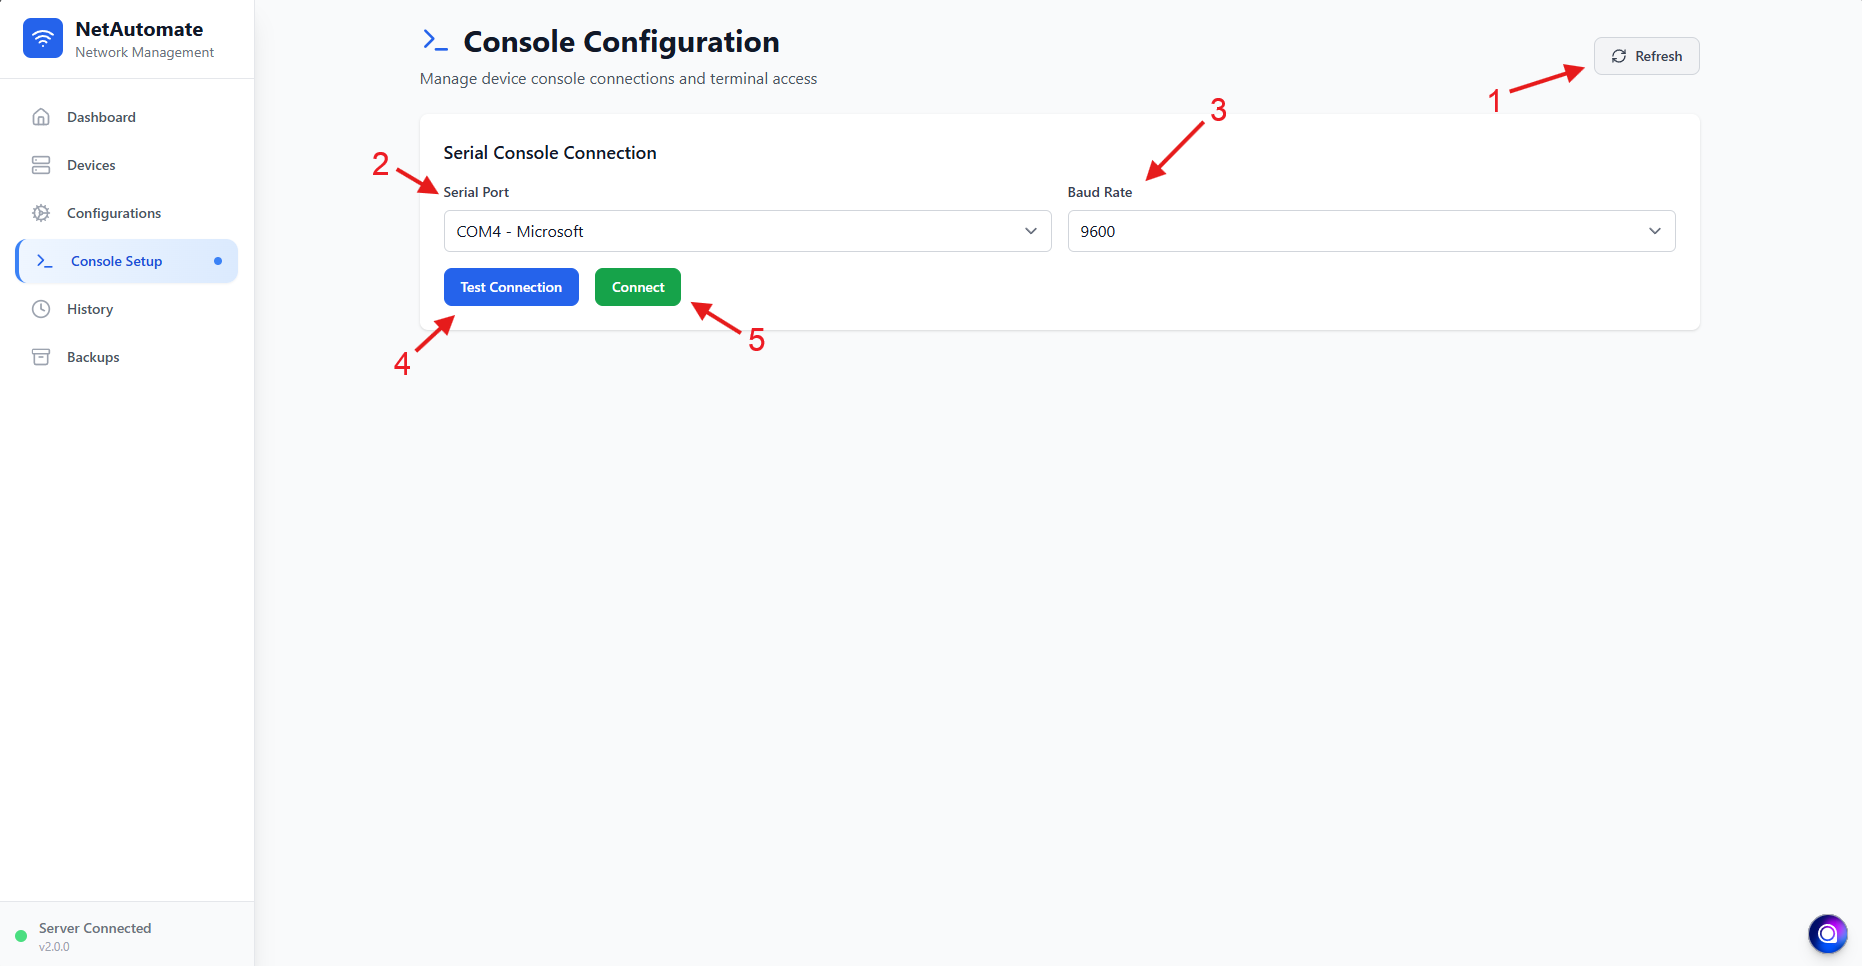
\includegraphics[width=1.0\textwidth]{Image/ConsoleSetup.png}
}
\caption{\fontSixTeen{หน้าจอ Console Configuration}}
\label{fig4:ConsoleSetup}
\end{figure}

\hspace*{1.3em} %ย่อหน้า
จากภาพที่ \ref{fig4:ConsoleSetup} แสดงหน้าจอสำหรับ Console Configuration สำหรับการกำหนดค่าอุปกรณ์ SSH ซึ่งประกอบด้วยฟิลด์ต่าง ๆ  ดังนี้

\hspace*{1.3em} %ย่อหน้า
หมายเลข 1 ปุ่มรีเฟรช (Refresh) เพื่อดึงข้อมูลอุปกรณ์ล่าสุดจากฐานข้อมูล

\hspace*{1.3em}
หมายเลข 2 เลือก Serial Port ที่เชื่อมต่อกับอุปกรณ์

\hspace*{1.3em}
หมายเลข 3 เลือก Baud Rate ที่ใช้ในการเชื่อมต่อกับอุปกรณ์

\hspace*{1.3em}
หมายเลข 4 ปุ่ม Test Connection กับอุปกรณ์ผ่านสาย Serial

\hspace*{1.3em}
หมายเลข 5 ปุ่ม Connect กับอุปกรณ์ผ่านสาย Serial

\begin{figure}[H]
\centering
\adjustbox{frame, width=1.0\textwidth}{%สร้างกรอบของภาพ
    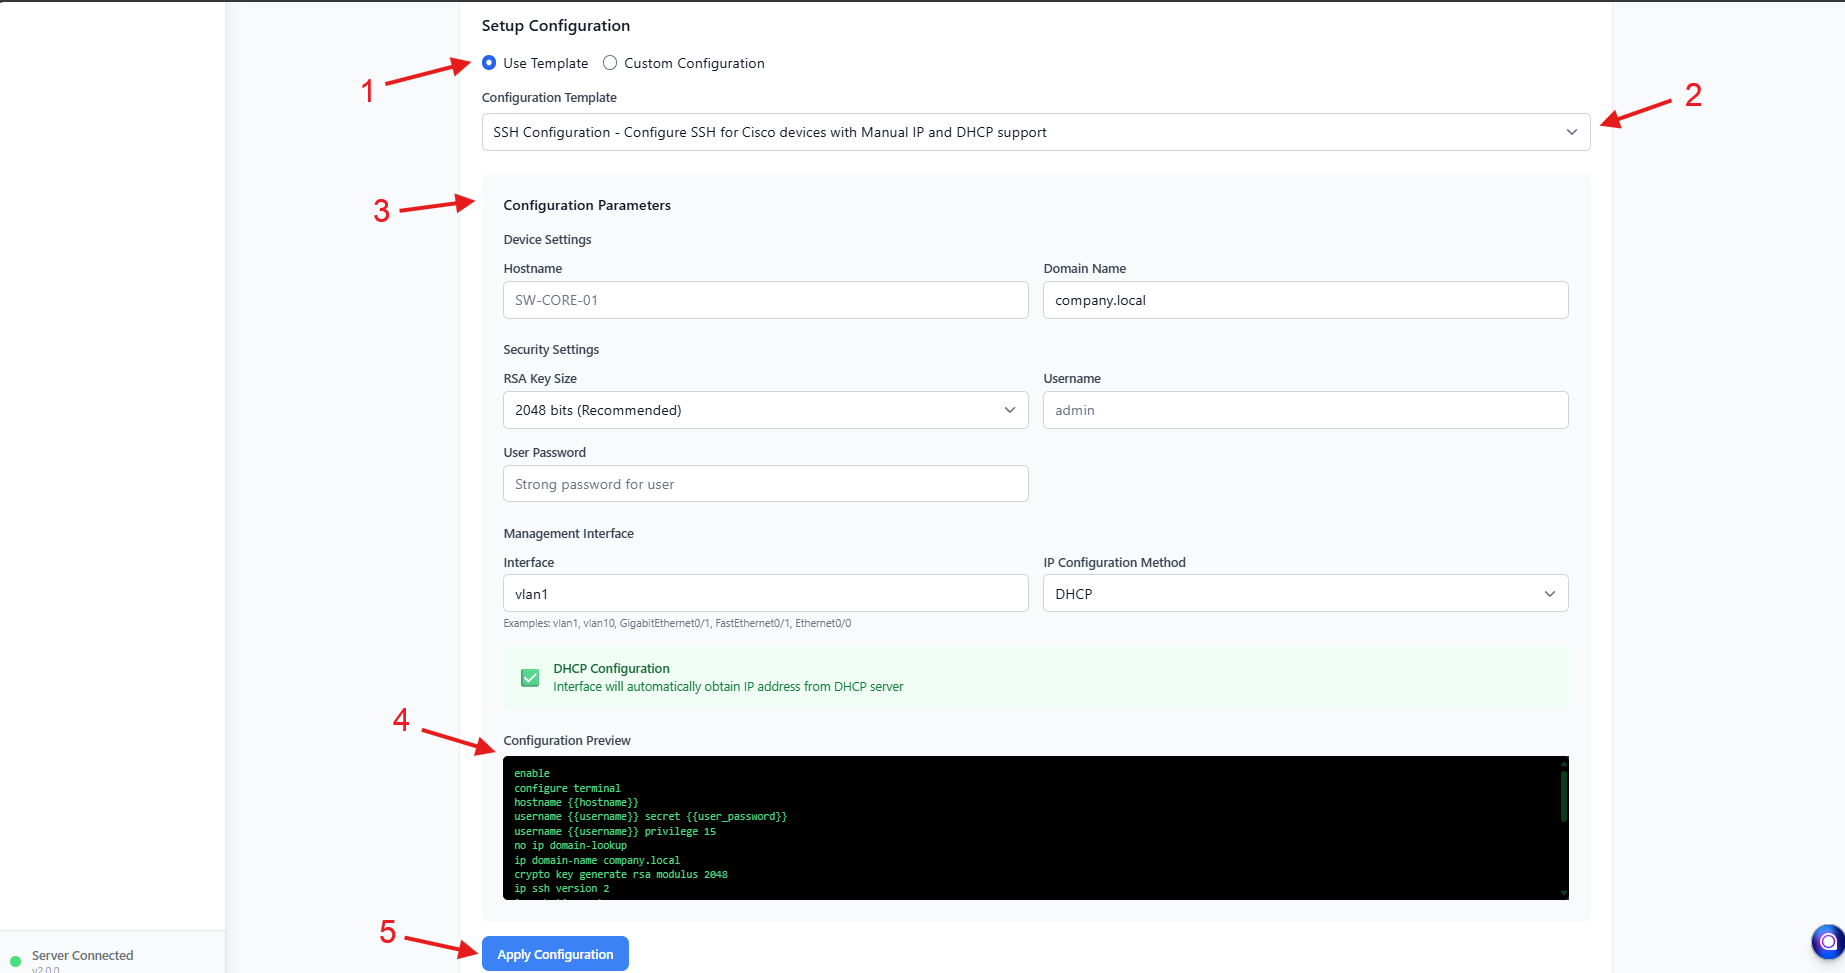
\includegraphics[width=1.0\textwidth]{Image/ConsoleSetup1.png}
}
\caption{\fontSixTeen{หน้าจอ Console Configuration (ต่อ)}}
\label{fig4:ConsoleSetup1}
\end{figure}

\hspace*{1.3em} %ย่อหน้า
จากภาพที่ \ref{fig4:ConsoleSetup1} แสดงหน้าจอสำหรับ Console Configuration สำหรับการกำหนดค่าอุปกรณ์ SSH ซึ่งประกอบด้วยฟิลด์ต่าง ๆ  ดังนี้

\hspace*{1.3em} %ย่อหน้า
หมายเลข 1 เลือกโหมดที่ต้องการแบบ Template หรือ Custom

\hspace*{1.3em}
หมายเลข 2 เลือก Template ที่ต้องการใช้ในการตั้งค่าอุปกรณ์

\hspace*{1.3em}
หมายเลข 3 ระบุค่าต่าง ๆ ที่ต้องการตั้งค่าอุปกรณ์ ซึ่งค่าที่ระบุจะขึ้นอยู่กับ Template ที่เลือก

\hspace*{1.3em}
หมายเลข 4 ฟิลด์แสดง Configuration Preview ที่จะถูกคอนฟิกให้กับอุปกรณ์

\hspace*{1.3em}
หมายเลข 5 ปุ่ม Apply Configuration เพื่อส่งคอนฟิกที่สร้างขึ้นไปยังอุปกรณ์

\begin{figure}[H]
\centering
\adjustbox{frame, width=1.0\textwidth}{%สร้างกรอบของภาพ
    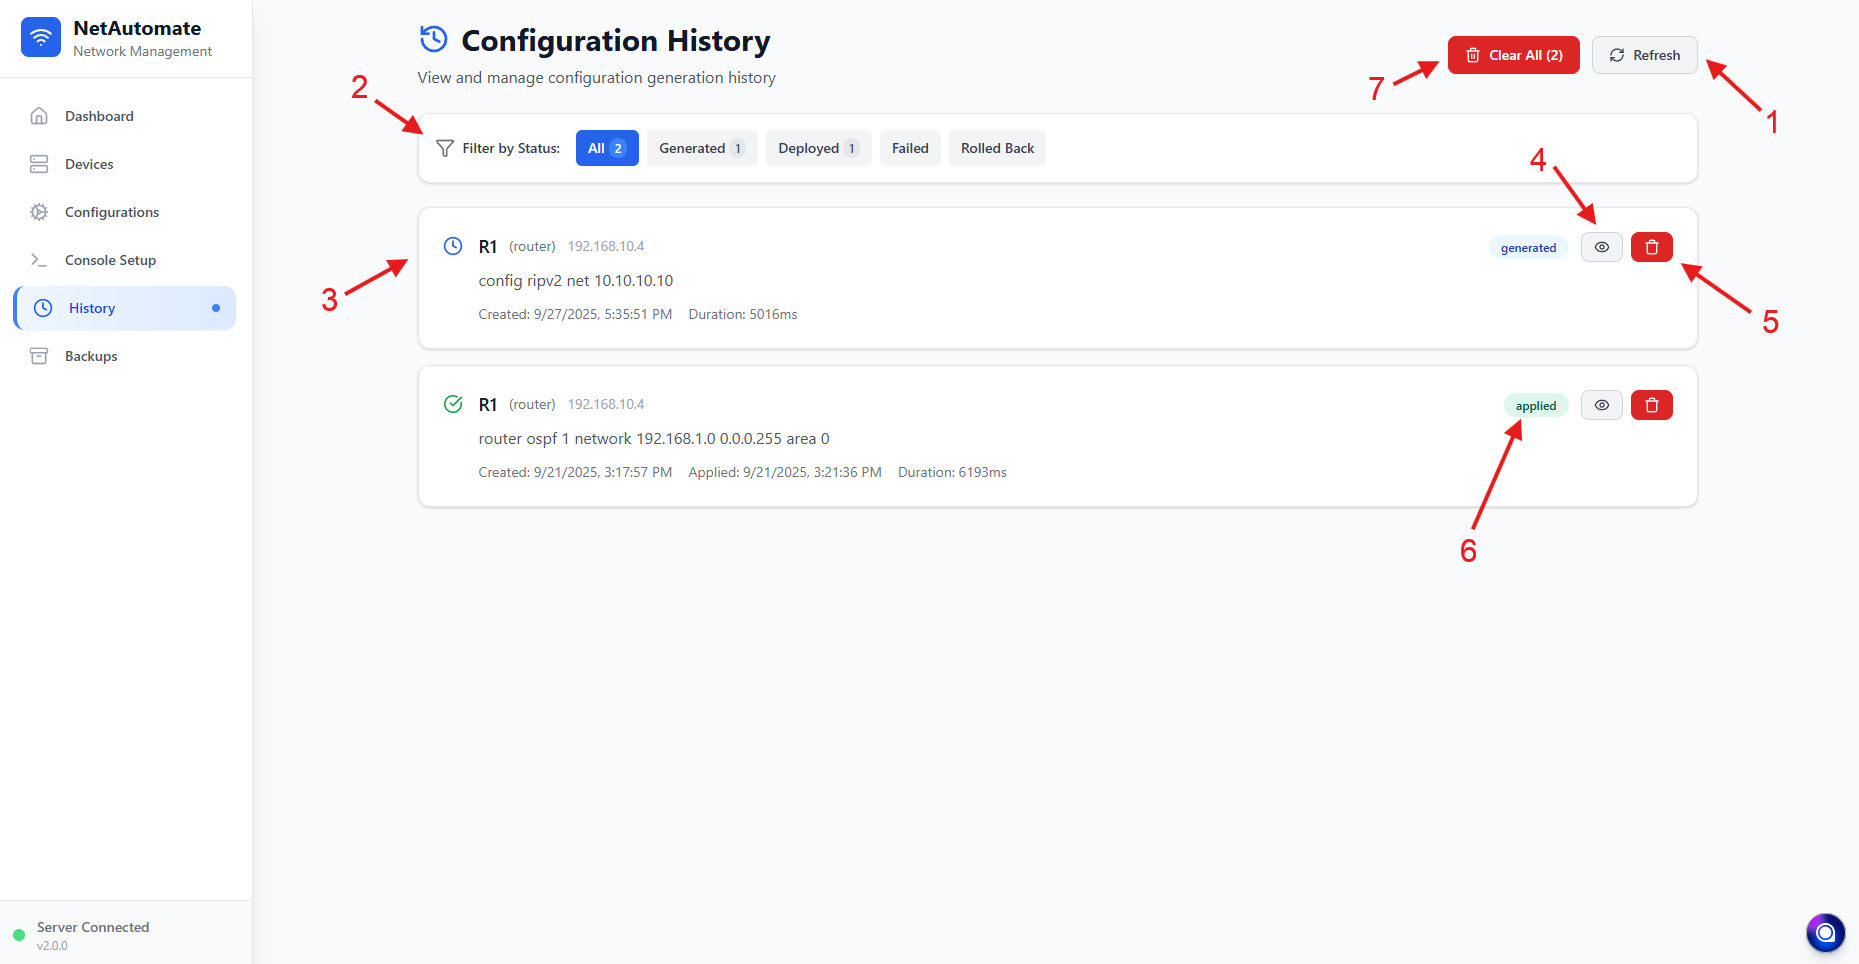
\includegraphics[width=1.0\textwidth]{Image/History.png}
}
\caption{\fontSixTeen{หน้าจอ Configuration History}}
\label{fig4:History}
\end{figure}

\hspace*{1.3em} %ย่อหน้า
จากภาพที่ \ref{fig4:History} แสดงหน้าจอสำหรับ Configuration History ซึ่งประกอบด้วยฟิลด์ต่าง ๆ  ดังนี้

\hspace*{1.3em} %ย่อหน้า
หมายเลข 1 ปุ่มรีเฟรช (Refresh) เพื่อดึงข้อมูลอุปกรณ์ล่าสุดจากฐานข้อมูล

\hspace*{1.3em}
หมายเลข 2 Filter ข้อมูลอุปกรณ์ที่ต้องการดูประวัติการกำหนดค่ามี 4 ตัวเลือก ได้แก่ Generated, Deployed, Failed, Rolled Back

\hspace*{1.3em}
หมายเลข 3 แสดงรายการและรายละเอียดแบบย่อของ Configuration 

\hspace*{1.3em}
หมายเลข 4 ปุ่มแสดงรายละเอียดของ Configuration ที่ LLM Generate ออกมา

\hspace*{1.3em}
หมายเลข 5 ปุ่มลบ (Delete) สำหรับลบ Configuration ที่เลือกออกจากระบบ

\hspace*{1.3em}
หมายเลข 6 แสดงสถานะของ Configuration ที่เลือก

\hspace*{1.3em}
หมายเลข 7 ปุ่มลบทั้งหมด (Clear All) สำหรับลบ Configuration ทั้งหมดออกจากระบบ


\begin{figure}[htbp]
\centering
\adjustbox{frame, width=1.0\textwidth}{%สร้างกรอบของภาพ
    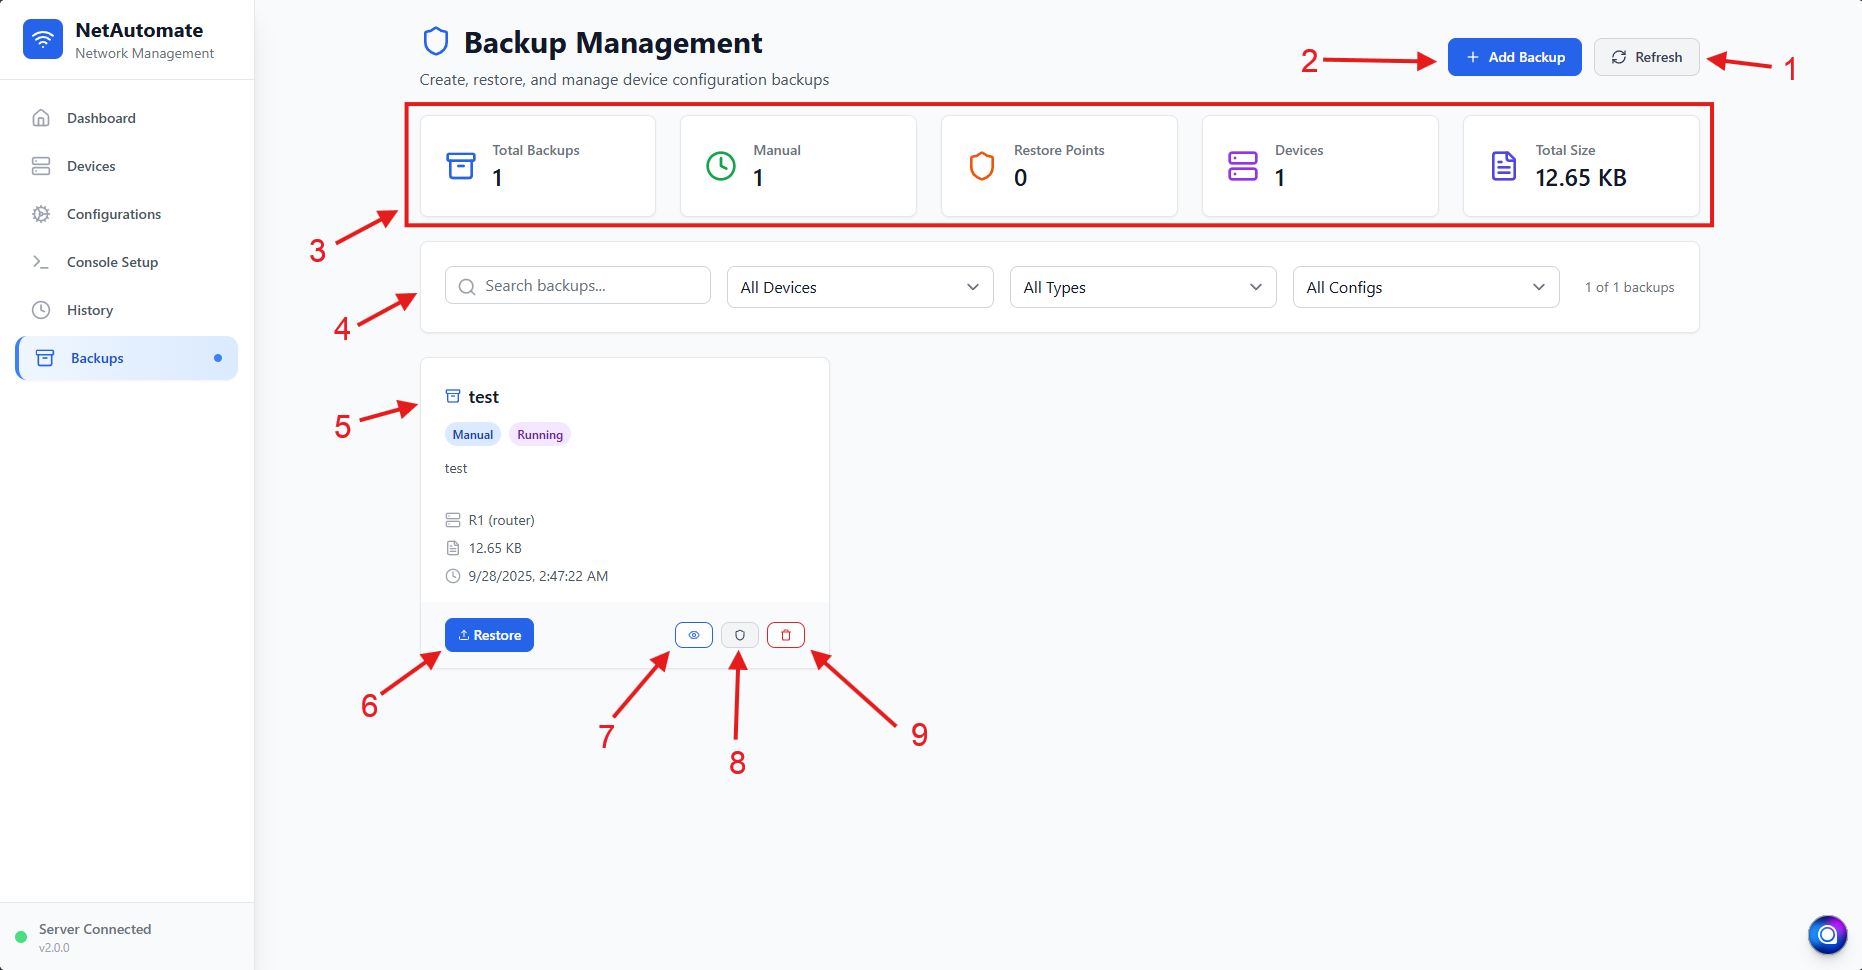
\includegraphics[width=1.0\textwidth]{Image/Backup.png}
}
\caption{\fontSixTeen{หน้าจอ Backup Configuration}}
\label{fig4:Backup}
\end{figure}
\hspace*{1.3em} %ย่อหน้า

\hspace*{1.3em} %ย่อหน้า

\hspace*{1.3em} %ย่อหน้า

\hspace*{1.3em} %ย่อหน้า

\hspace*{1.3em} %ย่อหน้า

\hspace*{1.3em} %ย่อหน้า

\hspace*{1.3em} %ย่อหน้า
จากภาพที่ \ref{fig4:Backup} แสดงหน้าจอสำหรับ Backup Configuration ซึ่งประกอบด้วยฟิลด์ต่าง ๆ  ดังนี้

\hspace*{1.3em} %ย่อหน้า
หมายเลข 1 ปุ่มรีเฟรช (Refresh) เพื่อดึงข้อมูลอุปกรณ์ล่าสุดจากฐานข้อมูล

\hspace*{1.3em}
หมายเลข 2 ปุ่มเ Add Backup เพื่อสำรองข้อมูลการกำหนดค่าปัจจุบันของอุปกรณ์

\hspace*{1.3em}
หมายเลข 3 แสดงรายละเอียดจำนวน Total Backup, Total Backup Type, Device, Restore Point, Total Size

\hspace*{1.3em}
หมายเลข 4 Search Bar และ Filter สำหรับค้นหา Backup Configuration 

\hspace*{1.3em}
หมายเลข 5 แสดงรายการและรายละเอียดแบบย่อของ Backup Configuration

\hspace*{1.3em}
หมายเลข 6 ปุ่ม Restore สำหรับคืนค่าการกำหนดค่ากลับไปยังจุดที่สำรองข้อมูลไว้

\hspace*{1.3em}
หมายเลข 7 ปุ่ม Preview สำหรับแสดง Configuration ที่สำรองข้อมูลไว้

\hspace*{1.3em}
หมายเลข 8 ปุ่ม Restore Point สำหรับแสดงจุดที่สำรองข้อมูลไว้

\hspace*{1.3em}
หมายเลข 9 ปุ่มลบ (Delete) สำหรับลบ Backup Configuration ที่เลือกออกจากระบบ

\section{การแก้ไขปัญหาทางเทคนิคที่สำคัญ}
\hspace*{1.3em}
ในระหว่างการพัฒนาและทดสอบระบบ พบปัญหาทางเทคนิคที่สำคัญหลายประการซึ่งได้รับการแก้ไขเพื่อให้ระบบทำงานได้อย่างเสถียรบน Vercel Serverless ดังนี้

\subsection{การแก้ไขปัญหา NETCONF Auto-Connect บน Vercel Serverless}
\hspace*{1.3em}
เนื่องจาก Vercel Serverless Functions เป็นแบบ Stateless ทำให้ NETCONF connections ที่เก็บไว้ใน in-memory Map จะสูญหายเมื่อ Serverless Function instance ถูกปิดหรือเปลี่ยน instance ส่งผลให้การดำเนินการ NETCONF เช่น get, get-config, rpc ล้มเหลวด้วยข้อผิดพลาด ``Not connected via NETCONF''

\hspace*{1.3em}
วิธีแก้ไข:
\begin{mycustomitem2}
    \item เพิ่มฟังก์ชัน \texttt{ensureConnected()} ใน NetconfHandler ของ Desktop Agent เพื่อตรวจสอบและเชื่อมต่อ NETCONF อัตโนมัติก่อนดำเนินการทุกครั้ง
    \item เพิ่มฟังก์ชัน \texttt{isConnected()} สำหรับตรวจสอบสถานะการเชื่อมต่อ
    \item Backend ส่ง Device Credentials (host, port, username, password) ไปพร้อมกับทุกคำสั่ง NETCONF เพื่อให้ Agent สามารถ Auto-Connect ได้
    \item เพิ่มระบบ Fallback ใน Backend ที่ตรวจสอบ Agent Online Status เมื่อ in-memory session หายไป
\end{mycustomitem2}

\subsection{การแก้ไขปัญหาการสำรองคอนฟิกด้วย Interactive Shell}
\hspace*{1.3em}
การสำรองข้อมูลคอนฟิกจากอุปกรณ์ Cisco ด้วยวิธี SSH exec เดิม ส่งคำสั่ง \texttt{terminal length 0} และ \texttt{show running-config} เป็นคำสั่งเดียว (\texttt{\\n} คั่น) ทำให้อุปกรณ์ Cisco ไม่สามารถประมวลผลคำสั่งได้ถูกต้องและส่งกลับข้อความผิดพลาดแทนคอนฟิกจริง

\hspace*{1.3em}
วิธีแก้ไข:
\begin{mycustomitem2}
    \item เพิ่มฟังก์ชัน \texttt{execBackupCommands()} ใน SSHHandler ที่ใช้ Interactive Shell แทน Single Exec
    \item ส่งคำสั่งแยกกันตามลำดับ พร้อม delay ระหว่างคำสั่ง (\texttt{terminal length 0} $\rightarrow$ delay $\rightarrow$ \texttt{show running-config})
    \item เพิ่มฟังก์ชัน \texttt{cleanConfig()} สำหรับทำความสะอาดผลลัพธ์ ลบ ANSI escape codes, Command Echo, Device Prompt และค้นหาจุดเริ่มต้นคอนฟิก (``Current configuration'' หรือ ``version'')
\end{mycustomitem2}

\subsection{การแก้ไขปัญหา Agent Relay Timeout สำหรับ Restore}
\hspace*{1.3em}
การ Restore คอนฟิกจาก Backup ประกอบด้วยหลายขั้นตอน: สร้าง Checkpoint Backup $\rightarrow$ Deploy คอนฟิก $\rightarrow$ บันทึกประวัติ ซึ่งใช้เวลารวมเกินกว่า Agent Relay maxWait เดิม (25 วินาที) ทำให้ระบบ Timeout และส่งกลับข้อผิดพลาด 500

\hspace*{1.3em}
วิธีแก้ไข:
\begin{mycustomitem2}
    \item เพิ่ม Agent Relay maxWait จาก 25 วินาที เป็น 55 วินาที (อยู่ภายใน Vercel 60 วินาที limit)
    \item เพิ่ม Deploy timeout จาก 25 วินาที เป็น 45 วินาที
    \item เพิ่มระบบ Extended Polling สำหรับ Restore ที่ตรวจสอบผลลัพธ์เพิ่มเติมหลัง Relay timeout
    \item ลด Checkpoint Backup timeout เหลือ 15 วินาที เพื่อเหลือเวลาสำหรับ Deploy
    \item รองรับสถานะ pending จาก Agent Relay แทนที่จะ throw error ทันที
\end{mycustomitem2}

\subsection{การแก้ไขปัญหา YANG Model Upload}
\hspace*{1.3em}
การอัปโหลด YANG Model ล้มเหลวด้วยข้อผิดพลาด 500 เนื่องจากสองสาเหตุ:

\hspace*{1.3em}
\textbf{(1) ปัญหาฝั่ง Client:} ช่อง Namespace มีการกำหนด \texttt{type="url"} ทำให้ HTML5 validation ไม่ยอมรับค่าที่ไม่ใช่ URL และไม่มีการตรวจสอบขนาดไฟล์ก่อนอัปโหลด

\hspace*{1.3em}
\textbf{(2) ปัญหาฝั่ง Server:} Auth Middleware ใช้ \texttt{.lean()} ในการ query ผู้ใช้จาก MongoDB ซึ่งส่งกลับ Plain JavaScript Object ไม่มี Mongoose Virtual Getter (\texttt{.id}) ทำให้ \texttt{req.user.id} เป็น \texttt{undefined} เมื่อนำไปบันทึก YANG Model ที่กำหนด \texttt{userId} เป็น required จะเกิด Mongoose ValidationError

\hspace*{1.3em}
วิธีแก้ไข:
\begin{mycustomitem2}
    \item เปลี่ยน \texttt{type="url"} เป็น \texttt{type="text"} สำหรับช่อง Namespace
    \item เพิ่มการตรวจสอบขนาดไฟล์ไม่เกิน 4MB (ขีดจำกัดของ Vercel Hobby Plan)
    \item เปลี่ยน \texttt{req.user.id} เป็น \texttt{req.userId} ในทุก Route ของ YANG Models (8 จุด) ซึ่ง \texttt{req.userId} ถูกกำหนดค่าในn Auth Middleware จาก \texttt{user.\_id} โดยตรง
\end{mycustomitem2}






































